%%
%% This is file `sample-sigconf.tex',
%% generated with the docstrip utility.
%%
%% The original source files were:
%%
%% samples.dtx  (with options: `sigconf')
%% 
%% IMPORTANT NOTICE:
%% jj
%% For the copyright see the source file.
%% 
%% Any modified versions of this file must be renamed
%% with new filenames distinct from sample-sigconf.tex.
%% 
%% For distribution of the original source see the terms
%% for copying and modification in the file samples.dtx.
%% 
%% This generated file may be distributed as long as the
%% original source files, as listed above, are part of the
%% same distribution. (The sources need not necessarily be
%% in the same archive or directory.)
%%
%% The first command in your LaTeX source must be the \documentclass command.
\documentclass[sigconf]{acmart}

\usepackage[scheme=plain]{ctex}
\renewcommand{\abstractname}{摘要}
\usepackage{booktabs} % For formal tables
% \usepackage[colorinlistoftodos]{todonotes}
\usepackage{algorithmic}
\usepackage[linesnumbered, ruled, vlined]{algorithm2e}
\usepackage{multirow}
\usepackage{tablefootnote}
\usepackage{graphicx}
\usepackage{subfigure}
\usepackage{flushend}
\usepackage{color}
\usepackage{enumitem}
\usepackage{array, makecell}
\usepackage{footmisc}
\usepackage{amsmath}
\usepackage{amssymb}
\let\Bbbk\relax         %%redefined in newtxmath.sty
% \usepackage{ulem} 
\usepackage{xcolor}
\newcommand\yang[1]{\textcolor{magenta}{[Hongxia: #1]}}
\newcommand\blue[1]{\textcolor{blue}{#1}}
\newcommand\red[1]{\textcolor{blue}{#1}}
\newcommand\zc[1]{\textcolor{blue}{[zc: #1]}}
\newcommand\xz[1]{\textcolor{teal}{[xz: #1]}}
% \newcommand\hide[1]{}
\newcommand\green[1]{\textcolor{green}{#1}}
\newcommand{\hide}[1]{}
\newcommand{\jie}[1]{\textbf{\color{red}[(JT: #1 )]}}  % to fix
\newcommand{\vpara}[1]{\vspace{0.07in}\noindent\textbf{#1 }}
\newcommand{\model}{{ComiRec}}

\newtheorem{definition}{Definition}
\newtheorem{problem}{Problem}


%%
%% \BibTeX command to typeset BibTeX logo in the docs
\AtBeginDocument{%
  \providecommand\BibTeX{{%
    \normalfont B\kern-0.5em{\scshape i\kern-0.25em b}\kern-0.8em\TeX}}}

%% Rights management information.  This information is sent to you
%% when you complete the rights form.  These commands have SAMPLE
%% values in them; it is your responsibility as an author to replace
%% the commands and values with those provided to you when you
%% complete the rights form.

\copyrightyear{2020}
\acmYear{2020}
\setcopyright{acmcopyright}
\acmConference[KDD '20]{Proceedings of the 26th ACM SIGKDD Conference on Knowledge Discovery and Data Mining}{August 23--27, 2020}{Virtual Event, CA, USA}
\acmBooktitle{Proceedings of the 26th ACM SIGKDD Conference on Knowledge Discovery and Data Mining (KDD '20), August 23--27, 2020, Virtual Event, CA, USA}
\acmPrice{15.00}
\acmDOI{10.1145/3394486.3403344}
\acmISBN{978-1-4503-7998-4/20/08}

%% These commands are for a PROCEEDINGS abstract or paper.

%%
%% Submission ID.
%% Use this when submitting an article to a sponsored event. You'll
%% receive a unique submission ID from the organizers
%% of the event, and this ID should be used as the parameter to this command.
%%\acmSubmissionID{123-A56-BU3}

%%
%% The majority of ACM publications use numbered citations and
%% references.  The command \citestyle{authoryear} switches to the
%% "author year" style.
%%
%% If you are preparing content for an event
%% sponsored by ACM SIGGRAPH, you must use the "author year" style of
%% citations and references.
%% Uncommenting
%% the next command will enable that style.
%%\citestyle{acmauthoryear}

%%
%% end of the preamble, start of the body of the document source.
\settopmatter{printacmref=true}

\begin{document}

\fancyhead{}

%%
%% The "title" command has an optional parameter,
%% allowing the author to define a "short title" to be used in page headers.
\title{可控的多兴趣推荐框架}
% \title{Controllable Multi-Interest Sequential Recommendation}

\author[Y. Cen, J. Zhang, X. Zou, C. Zhou, H. Yang and J. Tang]{
    Yukuo Cen$^{\dagger}$, Jianwei Zhang$^{\ddagger}$, Xu Zou$^{\dagger}$, Chang Zhou$^{\ddagger}$, Hongxia Yang$^{\ddagger*}$, Jie Tang$^{\dagger*}$
}
\affiliation{
    $^\dagger$ Department of Computer Science and Technology, Tsinghua University
}
\affiliation{
    $^\ddagger$ DAMO Academy, Alibaba Group
}
\email{
  {cyk18, zoux18}@mails.tsinghua.edu.cn
}
\email{
  {zhangjianwei.zjw, ericzhou.zc, yang.yhx}@alibaba-inc.com
}
\email{
  jietang@tsinghua.edu.cn
}


%%
%% By default, the full list of authors will be used in the page
%% headers. Often, this list is too long, and will overlap
%% other information printed in the page headers. This command allows
%% the author to define a more concise list
%% of authors' names for this purpose.
\renewcommand{\authors}{Yukuo Cen, Jianwei Zhang, Xu Zou, Chang Zhou, Hongxia Yang and Jie Tang}
\renewcommand{\shortauthors}{Y. Cen et al.}


%%
%% The abstract is a short summary of the work to be presented in the
%% article.
\begin{abstract}
\renewcommand{\thefootnote}{\fnsymbol{footnote}}
\footnotetext[1]{Hongxia Yang 和 Jie Tang 是通讯作者.}
\renewcommand{\thefootnote}{\arabic{footnote}}


最近,由于深度学习的快速发展,神经网络已广泛用于电子商务推荐系统。
我们将推荐器系统形式化为顺序推荐问题,旨在预测与用户进行交互的下一个项目。
近期的研究工作通常会根据用户的行为顺序进行整体嵌入。但是,统一的用户嵌入无法反映该用户在一段时间内的多重兴趣。
在本文中,我们为顺序推荐提出了一种新颖的可控多兴趣框架(\textbf{\textit{co}}ntrollable \textbf{\textit{m}}ulti-\textbf{\textit{i}}nterest framework for the sequential \textbf{\textit{rec}}ommendation),称为 \model。我们的多兴趣模块从用户行为序列中捕获多个兴趣,可将其用于从大型项目池中检索候选项目。然后将这些项目输入汇总模块以获取总体推荐。聚合模块利用可控因素来平衡推荐准确性和多样性。
我们针对两个现实世界的数据集,亚马逊和淘宝,进行了顺序推荐的实验。实验结果表明,我们的框架相对于时下最先进的模型\footnote{代码可以在 \url{https://github.com/THUDM/ComiRec} 找到}有了显着改进。
我们的框架也已成功部署在离线阿里巴巴分布式云平台上。
\end{abstract}

%%
%% The code below is generated by the tool at http://dl.acm.org/ccs.cfm.
%% Please copy and paste the code instead of the example below.
%%
\begin{CCSXML}
<ccs2012>
<concept>
<concept_id>10002951.10003317.10003347.10003350</concept_id>
<concept_desc>Information systems~Recommender systems</concept_desc>
<concept_significance>500</concept_significance>
</concept>
<concept>
<concept_id>10010147.10010257.10010293.10010294</concept_id>
<concept_desc>Computing methodologies~Neural networks</concept_desc>
<concept_significance>500</concept_significance>
</concept>
</ccs2012>
\end{CCSXML}

\ccsdesc[500]{信息系统~推荐系统}
\ccsdesc[500]{计算方法~神经网络}

%%
%% Keywords. The author(s) should pick words that accurately describe
%% the work being presented. Separate the keywords with commas.
\keywords{推荐系统; 顺序推荐; 多兴趣网络}

%%
%% This command processes the author and affiliation and title
%% information and builds the first part of the formatted document.
\maketitle

\section{引言}\label{sec:intro}
% !TEX root = ./0.main.tex

电子商务的发展近年来改变了我们的购物方式。推荐系统在电子商务公司中起着基础的作用。
传统的推荐方法主要使用协作过滤方法~\cite{sarwar2001item,schafer2007collaborative} 来预测用户和项目之间的得分。 最近,由于深度学习的快速发展,神经网络已广泛用于电子商务推荐系统。 神经推荐系统生成用户和项目的表示形式,且优于传统的推荐方法。但是,由于电子商务用户和商品的规模较大,因此很难使用深度模型直接给出每对用户和商品之间的点击率(CTR)预测。 目前的工业实践是使用快速k邻近算法 (例如, Faiss~\cite{JDH17}) 来生成候选项目,然后使用深度模型(例如, xDeepFM~\cite{lian2018xdeepfm}) 来集成用户和商品以优化业务指标(例如CTR)。

% \xz{The traditional way of building up such systems mainly relies on collaborative filters, while neural-network-based models are becoming more and more popular. Modern architecture first embeds users and items, then use fast matching algorithms like fast K nearest neighbors (Faiss~\cite{JDH17}) to match these embeddings, or use more complex ways that integrate the attributes of users and items to optimize the business metrics, like xDeepFM~\cite{lian2018xdeepfm}.  } 
% Recommender systems become a fundamental part of e-commerce companies. All sorts of recommendation algorithms play an essential role in recommender systems. Traditional recommendation methods mainly use collaborative filtering to predict scores between users and items and recommend users with high-score items. Recently, neural networks have been widely used in e-commerce recommender systems, which owe to the rapid development of deep learning. Neural recommendation methods generate representations for users and items and outperform traditional recommendation algorithms.

% As we can see, the function of neural networks is to obtain the item candidates instead of giving the final recommendation list for each user.
% \xz{The problem of neural-network-based models is that they require to run. If the number of users and items scale up tremendously, for example, billions of users and items, then there's still a large gap between embeddings and final recommendations.  } 
% Excessive item pool with billions of items limits the effects of neural networks. 
最近的一些工作利用图嵌入方法来获取用户和项目的表示,这些表示可用于下游应用程序。例如,PinSage~\cite{ying2018graph} 建立在 GraphSAGE~\cite{hamilton2017inductive} 的基础上,并将基于图卷积网络的方法应用于具有数十亿个节点和边的生产规模数据。GATNE~\cite{cen2019representation} 考虑了不同的用户行为类型,并利用异构图嵌入方法来学习用户和项目的表示。 但是,这种方法忽略了用户行为中的顺序信息,并且无法捕获相邻用户行为之间的相关性。 %Also, user behaviors are updated in real time, so recommendation methods should give real-time recommendations for all users. 

最近的研究~\cite{kang2018self,chen2018sequential,lv2019sdm} 将推荐系统形式化为顺序推荐问题。根据用户的行为历史记录,顺序推荐任务是预测他/她可能感兴趣的下一个项目。此任务反映了现实中的推荐系统的情况。许多最新模型可以根据其行为顺序为每个用户提供整体嵌入。但是,统一的用户嵌入很难代表多个兴趣。 例如,在图~\ref{fig:multiple_interest} 中,单击序列显示了Emma的三种不同兴趣。 作为一个现代女孩,Emma 对珠宝,手袋和化妆品感兴趣。 因此,在这段时间,她可能单击三个类别的项目。

% \begin{figure}
%     \centering
%     \includegraphics[width=0.45\textwidth]{figures/multiple_interests.pdf}
%     \caption{An example click sequence of a e-commerce user, Emma. The click sequence indicates that Emma has multiple interests including clothes, handbags, and makeups.}
%     \label{fig:multiple_interest}
% \end{figure}

\begin{figure*}
    \centering
    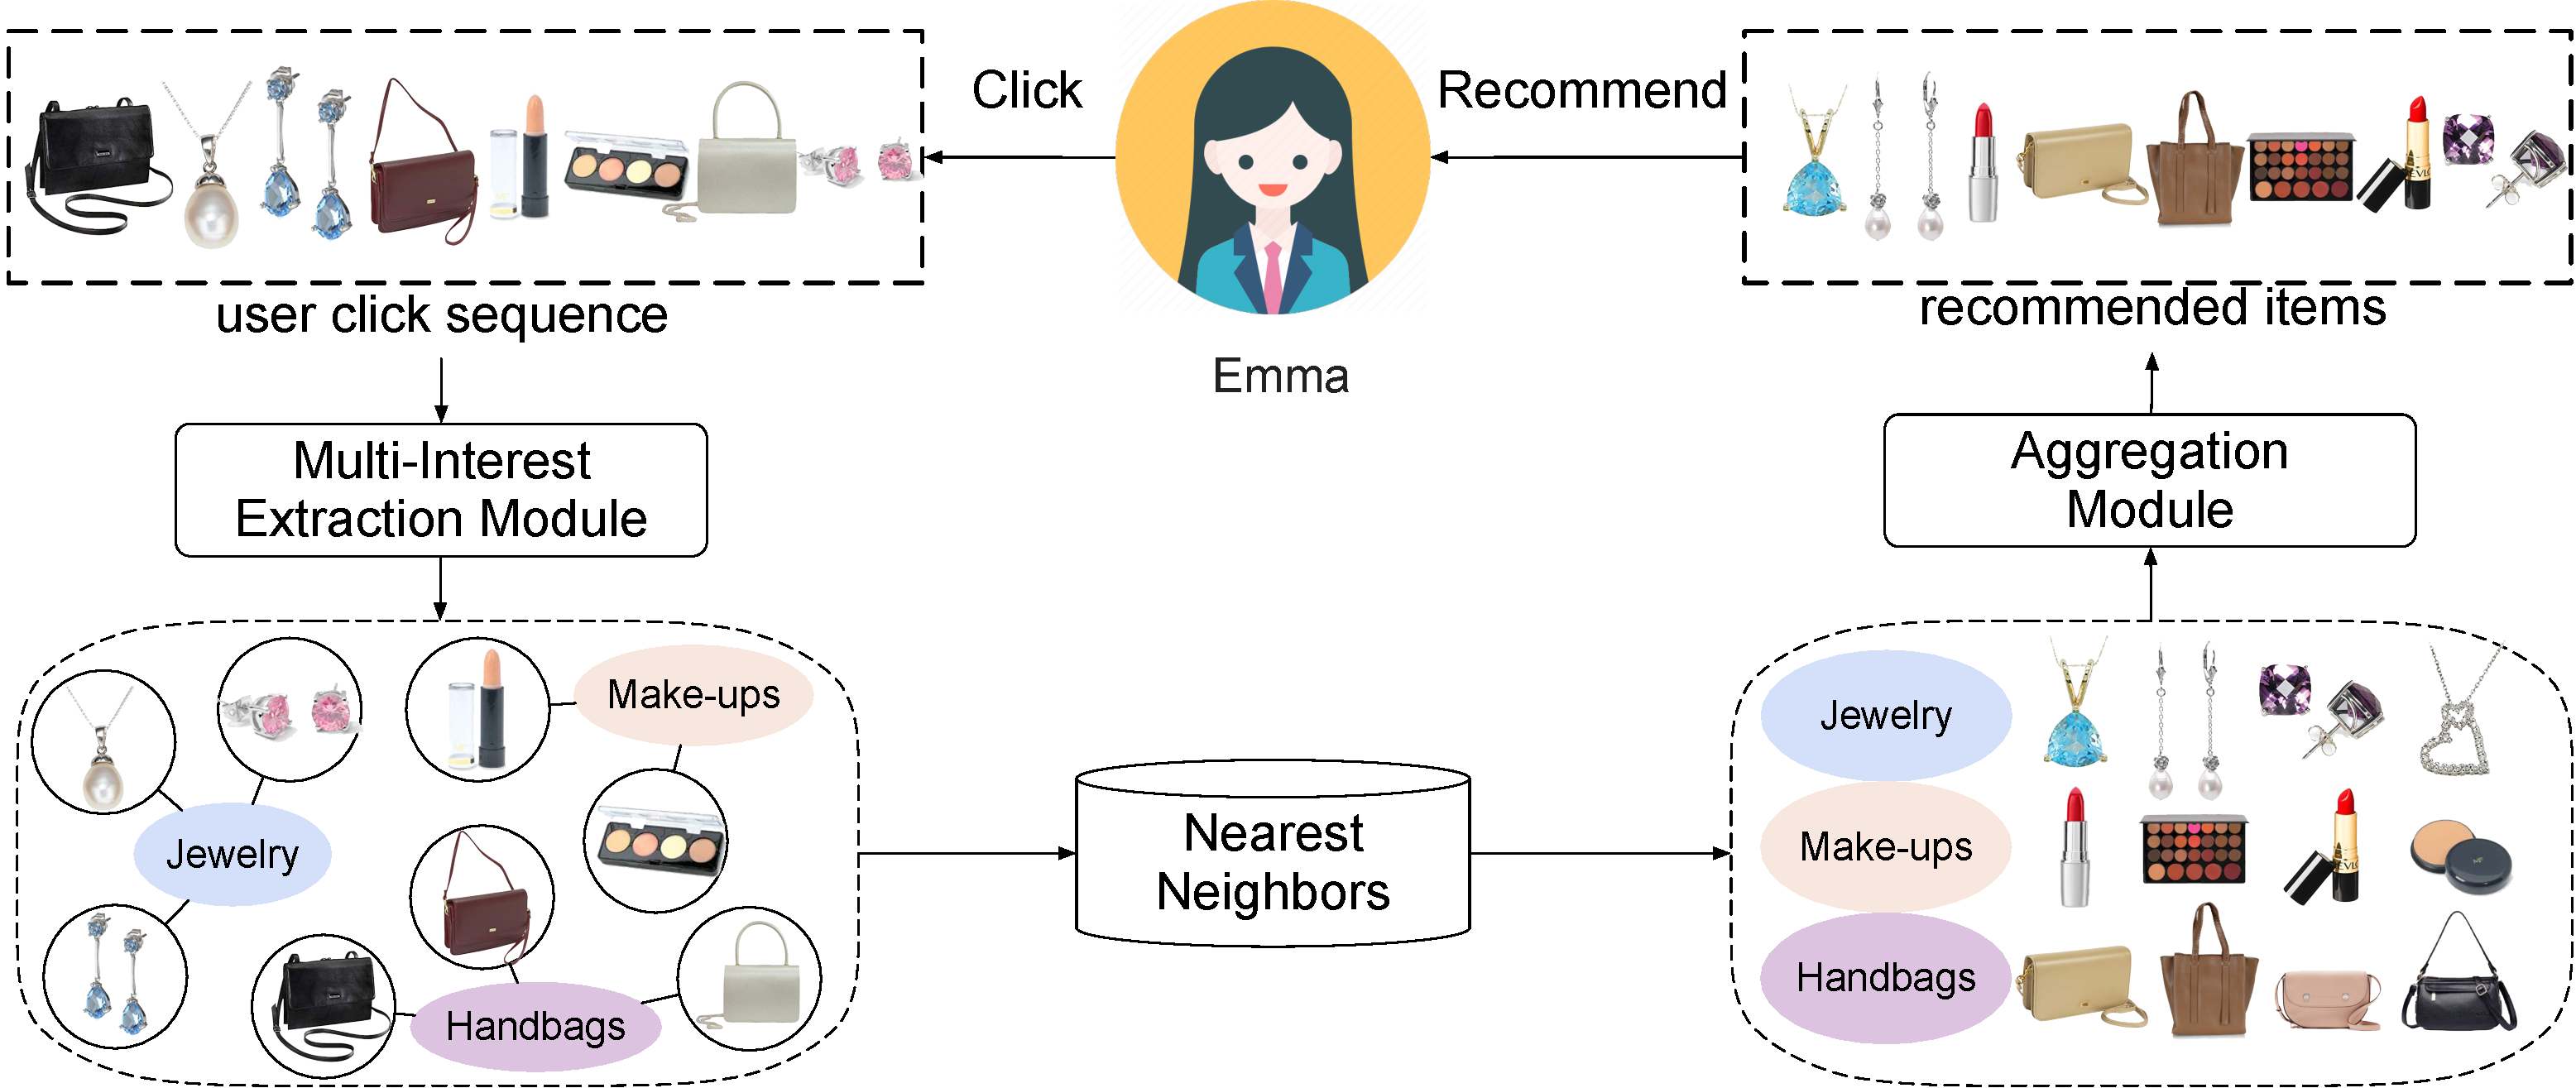
\includegraphics[width=0.8\textwidth]{figures/multi-interest-overview.pdf}
    \caption{我们提出的框架的一个令人振奋的例子。 电子商务平台用户Emma具有多种兴趣,包括珠宝,手袋和化妆品。 我们的多兴趣提取模块可以从她的点击序列中捕获这三个兴趣。 每个兴趣都基于兴趣嵌入独立地从大型项目池中检索项目。 汇总模块组合了来自不同兴趣的项目,并输出Emma推荐的总体前N个项目。 }
    \label{fig:multiple_interest}
\end{figure*}

在本文中,我们提出了一种新的可控多兴趣框架 \model。我们的多兴趣模块可以捕获用户的多个兴趣,可以将其用于检索候选项目。我们的汇总模块将这些来自不同兴趣的项目组合在一起,并输出总体建议。图~\ref{fig:multiple_interest} 显示了我们的多兴趣框架的一个令人振奋的例子。我们针对顺序推荐进行实验,这与我们的在线情况类似。实验结果表明,我们的框架优于其他最新模型。我们的框架也已成功部署在阿里巴巴分布式云平台上。十亿规模的工业数据集上的结果,进一步证实了我们的模型在实践中的有效性和效率。

总而言之,本文的主要贡献有:
\begin{itemize}
    \item 我们提出了一个综合框架,该框架将可控性和多兴趣组件集成在一个统一的推荐系统中。
    \item 我们通过实施和研究在线推荐方案来研究可控性在个性化系统上的作用。
    \item 我们的框架在两个具有挑战性的真实数据集上实现了最先进的性能,可进行顺序推荐。
\end{itemize}

\iffalse
\begin{itemize}
    \item We propose a novel controllable multi-interest framework based on user sequential behaviors for sequential recommendation.
    \item The controllable module in our framework can adjust the diversity of recommended item candidates. 
    % \item We adapt the capsule network with a variation of the dynamic routing method for the multi-interest extraction. 
    \item Our framework achieves state-of-the-art results on two real-world datasets for sequential recommendation.
    % \item CapsRec has been deployed on Alibaba recommender systems and significantly improves hit rate on a billion-scale industrial dataset. 
\end{itemize} 
\fi


% \vpara{Organization}
% The rest of the paper is organized as follows. Section~\ref{sec:related} summarizes related work. Section~\ref{sec:model} formulates the sequential recommendation problem and introduces our proposed framework in detail. In Section~\ref{sec:exp}, we conduct extensive experiments and case studies. Finally, we conclude in Section~\ref{sec:conclusion}.
%% vim: formatoptions=


\section{相关工作} \label{sec:related}
% !TEX root = ./0.main.tex

在本节中,我们介绍有关推荐系统和推荐多样性的相关文献,以及本文中使用的胶囊网络和注意力机制。
% we give the following three kinds of related literature, including neural recomemender systems, sequential recommendation, and capsule network. 

% \vpara{Recommender Systems.}
协作过滤~\cite{sarwar2001item,schafer2007collaborative} 方法已在现实世界的推荐系统中被证明是成功的,该系统可以查找相似的用户和项目并在此基础上进行推荐。 矩阵分解~\cite{koren2009matrix} 是经典推荐器研究中最流行的技术,它将用户和项都映射到联合潜因子空间,从而将用户-项目交互建模为该空间中的内积。 因子分解机(FMs)~\cite{rendle2010factorization}使用因子分解的参数对变量之间的所有交互进行建模,从而使在诸如推荐系统之类的稀疏问题中也可以估计交互。

\vpara{神经推荐系统.}
神经协作过滤(NCF)~\cite{he2017neural} 使用神经网络体系结构对用户和项目的潜在特征进行建模。
NFM~\cite{he2017nfm} 无缝结合了FM在建模二阶特征相互作用中的线性和神经网络在建模高阶特征相互作用中的非线性。
DeepFM~\cite{guo2017deepfm} 设计了一种端到端学习模型,该模型同时强调了CTR预测的低阶和高阶特征交互。
xDeepFM~\cite{lian2018xdeepfm} 扩展了DeepFM并可以显式学习特定有界度特征交互。
深度矩阵分解(DMF)~\cite{xue2017deep} 使用深度结构学习体系结构,基于显式评级和非偏好的隐式反馈,学习用于用户和项目表示的通用低维空间。
DCN~\cite{wang2017deep} 保留了深度模型的优点,并引入了一种新颖的交叉网络,该交叉网络在学习特定的有界度特征交互(bounded-degree feature interactions)时效率更高。
CMN~\cite{ebesu2018collaborative} 使用深度架构以非线性方式利用潜因子模型的全局结构和基于局部邻域的结构的优势来统一两类CF模型。


\vpara{序列推荐.}
顺序推荐是推荐系统的关键问题。关于推荐器系统的许多最新工作都集中在此问题上。FPMC~\cite{rendle2010factorizing} 包含用于购物车序列数据的正态矩阵分解模型和公共Markov链。HRM~\cite{wang2015learning} 扩展了FPMC模型,并采用了两层结构来构造来自上次交易的用户和项目的混合表示。GRU4Rec~\cite{hidasi2015session} 首先引入了一种基于RNN的方法来对整个会话进行建模,以获得更准确的建议。基于循环神经网络(RNN)的DREAM~\cite{yu2016dynamic}学习了用户的动态表示,以揭示用户的动态兴趣。Fossil~\cite{he2016fusing} 将基于相似度的方法与马尔可夫链平滑地集成在一起,以对稀疏和长尾数据集进行个性化的顺序预测。TransRec~\cite{he2017translation} 将项目嵌入向量空间,在该空间中,用户被建模为对项目序列进行操作的向量,以进行大规模顺序预测。RUM~\cite{chen2018sequential} 使用记忆增强的神经网络,并结合了协作过滤的见解来推荐建议。SASRec~\cite{kang2018self} 使用基于自注意力的序列模型来捕获长期语义,并使用注意力机制根据相对较少的动作进行预测。DIN~\cite{zhou2018deep} 设计了一个本地激活单元,以从过去针对某个广告的行为中自适应地学习用户兴趣的表示形式。SDM~\cite{lv2019sdm} 使用多头自注意力模块捕获多种类型的兴趣,并使用长短期门控融合模块合并长期偏好,从而对行为序列进行编码。

% DIEN~\cite{zhou2019deep} designs an interest extractor layer to capture temporal interests from history behavior sequence and an interest evolving layer to capture interest evolving process that is relative to the target item. DSIN~\cite{feng2019deep} leverages users' multiple historical sessions in their behavior sequences by Bi-LSTM and self-attention mechanism with bias encoding. 

\vpara{推荐多样性.}
研究人员已经意识到,仅遵循最准确的推荐方式可能不会获得最佳的推荐结果,因为最准确的结果往往会向用户推荐相似的项目,从而产生令人厌烦的推荐结果~\cite{panniello2014comparing}. 为了解决此类问题,推荐项目的多样性也起着重要的作用~\cite{slaney2006measuring}. 在多样性方面,有汇总的多样性~\cite{adomavicius2011improving},是指向用户推荐“长尾物品”的能力。许多研究集中于改善推荐系统的集合多样性~\cite{bag2019integrated,adomavicius2011improving,niemann2013new,qin2013promoting}. 其他工作着眼于推荐给个人用户的项目的多样性,即个人多样性~\cite{adomavicius2011improving,yu2019recommendation,kalaivanan2013recommendation,di2014analysis},这是指推荐给个人用户的项目之间的差异。

% In this paper, our system have the ability to balance between accuracy and individual diversity. However, the “individual diversity” in our model is not based on the traditional categorical diversity, but on the self-learnt interests for our model, making our work the first one to introduce the individual diversity on multiple interests of users. 
% \vpara{Transformer}
% Transformer~\cite{} has been widely used in NLP fields. Some researchers~\cite{} apply this architecture to the recommendation areas.

\vpara{注意力}
注意力机制可以追溯到几十年前的计算机视觉领域~\cite{burt1988attention,sun2003object}. 但在最近几年它才在机器学习的各个领域中普及。它首先由~\cite{bahdanau2014neural}引入机器翻译,后来成为一种叫做 \textit{tensor2tensor}~\cite{vaswani2017attention}的流行方法. BERT~\cite{devlin2018bert} 利用 \textit{tensor2tensor} 并在自然语言处理方面取得了巨大的成功。
% Since the sequential recommendation problem is similar in terms of formulation as the next word prediction problem for natural language processing, 
注意机制还适用于推荐系统~\cite{zhou2018atrank,cen2019representation},在现实世界中的推荐任务中非常有用。
% The attention mechanism in this paper follows the self-attention \cite{vaswani2017attention,zhou2018atrank} setting that we try to learn a scoring function according to the embedding themselves and assign weights by the calculated scores. 


\vpara{胶囊网络.}
“胶囊”的概念最早是由~\cite{hinton2011transforming} 提出的,并且在提出了动态路由方法 ~\cite{sabour2017dynamic} 之后就广为人知。
% ~\cite{e2018matrix} describes a version of capsules in which each capsule has a logistic unit to represent the presence of an entity and a 4$\times$4 matrix, which could learn to represent the relationship between the entity and the viewer. 
% ~\cite{kosiorek2019stacked} describes an unsupervised version of capsule networks, in which a neural encoder is used to infer the presence and poses of object capsules. 
MIND~\cite{li2019multi} 将胶囊网络引入推荐区域,并使用胶囊网络的动态路由机制捕获电商用户的多种兴趣,适用于对过去的行为进行聚类并提取各种兴趣。CARP~\cite{li2019capsule} 首先从用户和项目评论文档中提取观点和方面,然后根据其每个方面的观点和方面来推导每个逻辑单元的表示,以进行评分预测。

%% vim: formatoptions=


\section{方法}\label{sec:model}
% !TEX root = ./0.main.tex
在本节中,我们将阐述问题并详细介绍拟议的框架,并说明我们的框架与代表性的现有方法之间的区别。

\begin{table}
  \centering
  \caption{\label{tab:notation} 符号表.}
%   \small
%   \renewcommand{\arraystretch}{1.2}
  \begin{tabular}{c|p{2.55in}}
    \hline \hline
    \textbf{Notation} & \textbf{Description} \\
    \hline
    $u$ & 一个用户 \\
    $i$ & 一个项 \\
    $e$ & 一个交互 \\
    $\mathcal{U}$ & 用户集 \\
    $\mathcal{I}$ & 项集 \\
    % $\mathcal{E}$ & a user's sequence \\
    $\mathcal{I}_u$ & 用户的测试项集 $u$ \\
    % $\mathcal{D}$ & the set of training samples \\
    % $\mathcal{D}^{+/-}$ & the set of positive/negative training samples \\
    $d$ & 用户/项目嵌入的维度 \\
    $K$ & 兴趣嵌入的数量 \\
    $N$ & 候选项目数 \\
    $\mathbf{V}_u$ & 用户$u$ 的兴趣嵌入矩阵 \\
    $\delta(\cdot)$ & 指示函数 \\
    % $\mathbf{e}_i$ & the vector of primary capsule $i$ \\
    % $\mathbf{v}_j$ & the vector of interest capsule $j$ \\
    % $b_{ij}, c_{ij}$ & coupling coefficients of dynamic routing \\
    % $\mathbf{W}$ & transformation matrix \\
    \hline \hline
  \end{tabular}
\end{table}

\subsection{问题表述}
%~\cite{he2016fusing,hidasi2015session,rendle2010factorizing,smirnova2017contextual,tang2018personalized,tang2019towards}
% We formulate the \textit{sequential recommendation} problem as a sequence prediction problem. 
%recommend a set of items to each user that the user may be most interested in.
假设我们有一组用户 $u\in \mathcal{U}$ 和一组项目 $i\in \mathcal{I}$. 对于每个用户,我们都有一系列用户历史行为 $(e^{(u)}_{1}, e^{(u)}_{2}, \cdots, e^{(u)}_{n})$,按出现时间排序。$e^{(u)}_{t}$ 记录用户交互的第 $t^{th}$ 项。给定历史交互,\textit{顺序推荐}问题指预测用户可能会与之交互的下一个项目。
表~\ref{tab:notation} 中概述了用到的符号.

实际上,由于对延迟和性能的严格要求,工业推荐系统通常包括两个阶段,即匹配阶段和排名阶段。匹配阶段对应于检索前N个候选项目,而排名阶段用于按更精确的分数对候选项目进行排序。本文主要关注在匹配阶段提高有效性。在本节的以下部分中,我们将介绍可控制的多兴趣框架,并说明该框架对于\textit{顺序推荐}问题的重要性. % The overview of our models can be seen in Figure~\ref{fig:capsule}.

\begin{figure*}
    \centering
    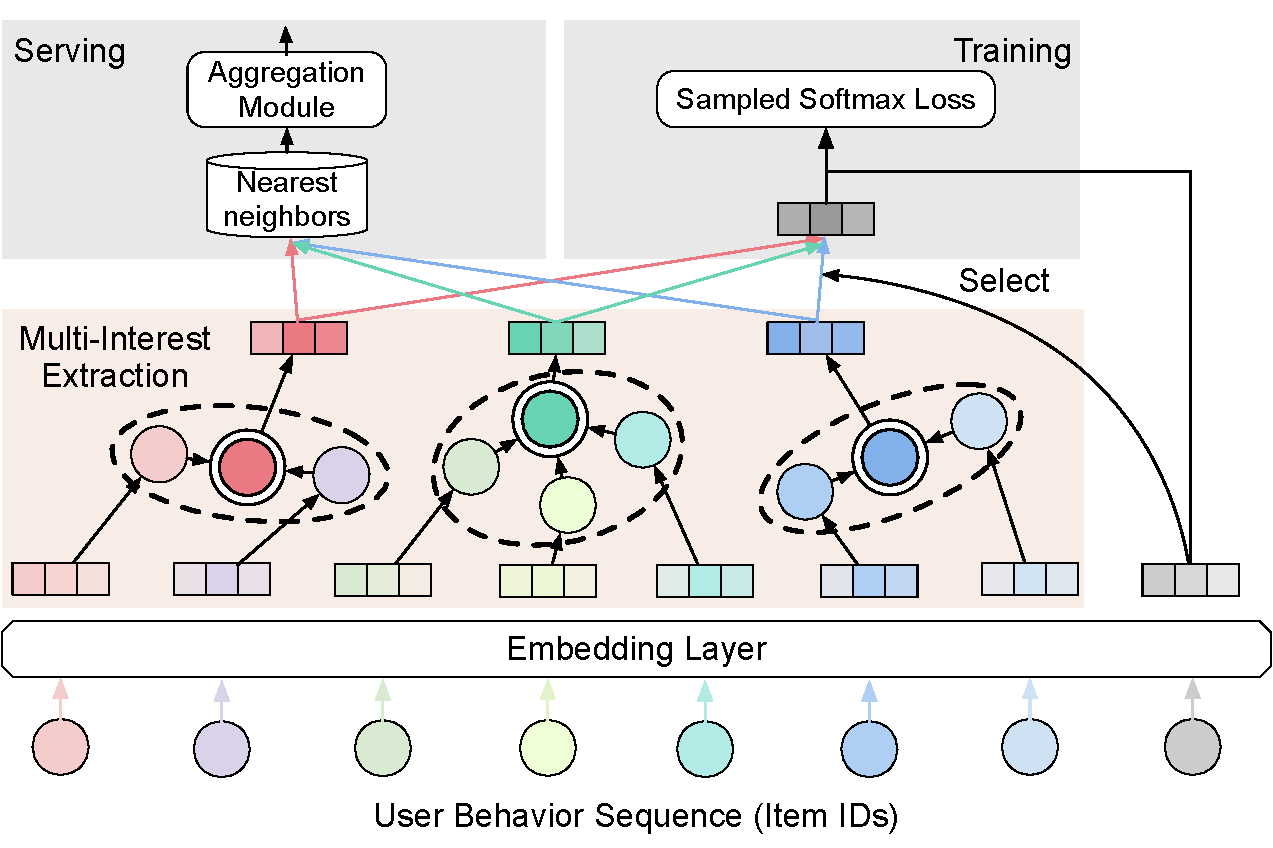
\includegraphics[width=0.8\textwidth]{figures/multi-interest-framework.pdf}
    \caption{顺序推荐模型的概述。我们模型的输入是用户行为序列,其中包含项ID的列表。该项目ID被送入嵌入层,并转化到该项目的嵌入。 兴趣嵌入是通过多兴趣提取模块生成的,然后可用于模型训练和服务。对于模型训练,将选择与目标嵌入最接近的兴趣嵌入来计算采样的softmax损失。为了提供服务,每个兴趣嵌入都将独立检索前N个最近的项目,然后将其馈入聚合模块。聚合模块通过可控制的过程来生成总体前N个项目,从而平衡推荐准确性和多样性。 }
    \label{fig:capsule_matching}
\end{figure*}

\subsection{多兴趣框架}
作为工业推荐系统的项目池通常由数百万甚至数十亿的项目,匹配阶段起着推荐系统至关重要的作用。 具体而言,匹配模型首先根据用户的历史行为来计算用户嵌入,然后基于用户嵌入为每个用户检索一组候选项目。借助快速K近邻算法(KNN)从大型项目池中选择最接近的项目以为每个用户生成候选集,我们主要集中在用户嵌入的计算上。换句话说,根据用户历史行为计算出的用户嵌入质量是匹配阶段的决定性因素。

现有的匹配模型通常使用RNN\cite{hidasi2015session,wu2017recurrent}为用户计算嵌入,但是大多数模型仅为每个用户生成一个嵌入向量。由于现实世界中的客户通常会考虑几种商品,而这些商品通常用于不同的用途,并且类别差异很大,因此,这种单一嵌入的方式缺乏足够的表达能力。 现实世界中客户的这种行为突显了需要使用多个向量来表示多重兴趣的重要性。基于这些考虑,我们为顺序推荐提出了一个多兴趣框架。我们框架的输入是用户行为序列,其中包含项目ID的列表,这些ID代表用户按时间顺序与商品的交互。商品ID被馈送到嵌入层,并转换为商品嵌入。多兴趣提取模块接收项目嵌入,并为每个用户生成多个兴趣。

%Interest capsules are generated through the dynamic routing method and can be then used for model training and online serving.

% RNN-based models~\cite{hidasi2015session,wu2017recurrent} are widely used in sequential recommendation. These models are effective for short-term user sequences~\cite{tang2019towards} but cannot capture long-term user interests from user sequences. 
要构建多兴趣提取模块,有很多可选的方法。 在本文中,我们探索了两种方法,即动态路由方法和自我关注方法,作为我们的多兴趣提取模块。 我们使用动态路由方法或自我关注方法的框架分别命名为 \model-DR 和 \model-SA.

\vpara{动态路由.}
%\zc{The motivation to exploit multi-interest network as the long-range model should be highlighted.}
我们将动态路由方法用作用户行为序列的多兴趣提取模块。 用户序列的项目嵌入可被视为主要胶囊,而多个用户兴趣可被视为兴趣胶囊。 我们使用CapsNet~\cite{sabour2017dynamic}中的动态路由方法. 
简要地说,我们使用动态路由来计算胶囊向量输入和输出。胶囊是一组神经元,其活动矢量代表特定类型的实体(例如对象或对象部件~\cite{sabour2017dynamic})的实例化参数。胶囊的输出矢量的长度表示由胶囊表示的实体在当前输入中的概率。令 $\mathbf{e}_i$ 为主要层的胶囊 $i$. 然后,我们基于主胶囊给出下一层胶囊 $j$ 的计算. 
%How to calculate capsules $\mathbf{v}_j$ of the output layer? 
我们首先将预测向量计算为
\begin{equation}
    \hat{\mathbf{e}}_{j|i}=\mathbf{W}_{ij} \mathbf{e}_{i},
\end{equation}
其中 $\mathbf{W}_{ij}$ 是转换矩阵。 那么,对胶囊 $j$ 的总输入就是所有预测矢量 $\hat{\mathbf{e}}_{j|i}$ 上的加权总和
\begin{equation}
        \mathbf{s}_j = \sum_i c_{ij} \hat{\mathbf{e}}_{j|i},
\end{equation}
其中 $c_{ij}$ 是由迭代动态路由过程确定的耦合系数。胶囊 $i$ 与下一层中所有胶囊之间的耦合系数总和为1. 我们使用初始 logits $b_{ij}$ 和“routing softmax”来计算耦合系数
\begin{equation}
    c_{ij}=\frac{\exp(b_{ij})}{\sum_k \exp(b_{ik})},
\end{equation}
其中 $b_{ij}$ 表示将胶囊 $i$ 和 $j$ 耦合的对数先验概率. 一个非线性“挤压”函数~\cite{sabour2017dynamic} 被提出来以确保短向量缩小到几乎为0的长度,长向量缩小到略小于1的长度. 胶囊 $j$ 的向量被计算为
\begin{equation}
    \label{eqn:squash}
    \mathbf{v}_j = \operatorname{squash}(\mathbf{s}_j) =  \frac{\|\mathbf{s}_j\|^2}{1+\|\mathbf{s}_j\|^2} \frac{\mathbf{s}_j}{\|\mathbf{s}_j\|},
\end{equation}
其中 $\mathbf{s}_j$ 是胶囊 $j$ 的总输入. 为了计算输出胶囊 $\mathbf{v}_j$, 我们需要根据 $\mathbf{v}_j$ 和 $\mathbf{e}_i$ 的内积来计算概率分布. $\mathbf{v}_j$ 的计算依赖与它自身;因此,动态路由方法被提出来解决这个问题. 整个动态路由过程在算法~\ref{algo:dynamic_routing}中给出. 然后用户 $u$ 的输出兴趣胶囊形成为下游任务的矩阵 $\mathbf{V}_u=[\mathbf{v}_1, ..., \mathbf{v}_K] \in \mathbb{R}^{d\times K}$.

% In order to ensure the diversity between interest capsules, we introduce a penalty term similar with \cite{lin2017structured}.

% \begin{equation}
%     P = \sum_{u\in \mathcal{U}}||\mathbf{V}_u \mathbf{V}_u^T-\mathbf{I}||_F^2
% \end{equation}
% where $||\cdot||_F$ denotes the Frobenius norm of a matrix. The penalty term $P$ will be multiplied by a coefficient and then added to the original loss (binary cross entropy loss or sampled softmax loss).

\begin{algorithm}[t]
	\caption{动态路由 \label{algo:dynamic_routing}}
	\KwIn{primary capsules $\mathbf{e}_i$, iteration times $r$, number of interest capsules $K$}
	\KwOut{interest capsules $\{\mathbf{v}_j, j=1,...,K\}$}
	for each primary capsule $i$ and interest capsule $j$: initialize $b_{ij} = 0$. \\
    \For{$iter = 1,\cdots,r$} {
        for each primary capsule $i$: $\mathbf{c}_i = \operatorname{softmax}(\mathbf{b}_{i})$.\\
        for each interest capsule $j$: $\mathbf{s}_j = \sum_{i} c_{ij}\mathbf{W}_{ij}\mathbf{e}_i$.\\%\hat{\mathbf{e}_{j|i}}$. \\

        for each interest capsule $j$: $\mathbf{v}_j = \operatorname{squash}(\mathbf{s}_j)$. \\

        for each primary capsule $i$ and interest capsule $j$: $b_{ij} = b_{ij}+ \mathbf{v}_j^\top \mathbf{W}_{ij}\mathbf{e}_i$.
    }
    \Return{$\{\mathbf{v}_j, j=1,...,K\}$}
\end{algorithm}


\vpara{自注意力方法.} 
自注意力方法~\cite{lin2017structured} 同样也可以被运用与我们的多兴趣提取模块。
给出用户的行为嵌入, $\mathbf{H}\in \mathbb{R}^{d\times n}$, 其中 $n$ 是用户序列的长度, 我们使用自注意力机制来获得一个权重向量 $\mathbf{a} \in \mathbb{R}^{n}$:
\begin{equation}
    \mathbf{a} = \operatorname{softmax}(\mathbf{w}_{2}^\top \operatorname{tanh}(\mathbf{W}_{1} \mathbf{H}))^\top,
\end{equation}
\noindent 其中 $\mathbf{w}_{2}$ 和 $\mathbf{W}_{1}$ 是可训练的参数,大小分别是为 $d_a$ 和 $d_a \times d$。 上标 $\top$ 表示向量或矩阵的转置。大小为 $n$ 的向量 $\mathbf{a}$ 表示用户行为的注意权重。 当根据注意力权重来总结用户行为的嵌入时,我们可以为用户获得向量表示 $\mathbf{v}_u = \mathbf{H} \mathbf{a}$ 。 对于利用用户序列顺序的自注意方法,我们将可训练的位置嵌入~\cite{vaswani2017attention} 添加到输入嵌入中。 位置嵌入与项目嵌入具有相同的尺寸 $d$ ,并且可以直接将两者相加。

该矢量表示关注并反映用户 $u$ 的特定兴趣。为了代表用户的整体兴趣,我们需要从关注不同兴趣的用户行为中获取多个 $\mathbf{v}_u$ 。因此,我们需要进行多次注意力。 我们将 $\mathbf{w}_{2}$ 扩展为 $\mathbf{W}_{2}$ 到 $d_a$-by-$K$ 的矩阵中。然后注意向量 $\mathbf{a}$ 变为注意矩阵 $\mathbf{A}$ 作为
\begin{equation}
    \mathbf{A} = \operatorname{softmax}(\mathbf{W}_{2}^\top \operatorname{tanh}(\mathbf{W}_{1} \mathbf{H}))^\top.
\end{equation}

用户兴趣最终矩阵 $\mathbf{V}_u$ 可以被这样计算
\begin{equation}
    \label{eqn:sa}
    \mathbf{V}_u = \mathbf{H} \mathbf{A}.
\end{equation}



\vpara{模型训练.}
在通过多兴趣提取模块根据用户行为计算出兴趣嵌入后,我们使用 \textit{argmax} 运算符为目标商品 $i$ 选择相应的用户嵌入向量:

\begin{equation}
    \label{eqn:argmax}
    \begin{aligned}
        % \mathbf{v}_u & = \operatorname{Attention}(\mathbf{e}_i, \mathbf{V}_u, \mathbf{V}_u) \\
        % & = \mathbf{V}_u \operatorname{softmax}(\mathbf{V}_u^\top \mathbf{e}_i),
        \mathbf{v}_u = \mathbf{V}_u[:, \operatorname{argmax}(\mathbf{V}_u^\top \mathbf{e}_i)],
    \end{aligned}
\end{equation}
其中 $\mathbf{e}_i$ 表示目标项目 $i$ 的嵌入,而 $\mathbf{V}_u$ 是由用户兴趣嵌入形成的矩阵 %The function $\operatorname{pow}$ is the element-wise exponential function and $p$ is a hyperparameter which controls the attention distribution. 

给定训练样本 $(u,i)$ ,用户嵌入 $\mathbf{v}_u$ ,项目嵌入 $\mathbf{e}_i$ ,我们可以计算用户 $u$ 与物品 $i$ 交互的可能性:

\begin{equation}
    \label{eqn:likelihood}
    P_\theta(i|u) = \frac{\exp(\mathbf{v}_u^\top \mathbf{e}_i)}{\sum_{k\in\mathcal{I}}\exp(\mathbf{v}_u^\top \mathbf{e}_k)}.
\end{equation}

我们模型的目标函数是最小化如下的负对数相似性

\begin{equation}
    \label{eqn:loss}
    loss = \sum_{u\in \mathcal{U}} \sum_{i\in \mathcal{I}_u} -\log P_\theta(i|u).
\end{equation}

方程 (\ref{eqn:likelihood}) 的和运算消耗很大;因此,我们用了一个简单的softmax方法 ~\cite{jean2014using, covington2016deep} 来训练我们的模型

\vpara{在线服务.}
对于在线服务,我们使用多兴趣提取模块为每个用户计算多个兴趣。 用户的每个兴趣向量都可以通过最近的邻居库(例如Faiss〜\ cite {JDH17})从大型项目池中独立检索前N个项目。 由多个兴趣检索的项目将被馈送到聚合模块中,以确定整体候选项目。 最后,将为用户推荐评分较高的项目。


% \subsection{Multi-Interest Extraction Module}


\begin{algorithm}[t]
	\caption{Greedy Inference \label{algo:贪心推断}}
	\KwIn{Candidate item set $\mathcal{M}$, number of output items $N$}
	\KwOut{Output item set $\mathcal{S}$}
	$\mathcal{S} = \varnothing$ \\
    \For{$iter = 1,\cdots,N$} {
        $j = \operatorname{argmax}_{i \in \mathcal{M} \backslash \mathcal{S}} \left( f(u, i) + \lambda \sum_{k \in \mathcal{S}} g(i,k) \right)$ \\
        $\mathcal{S} = \mathcal{S} \cup \{j\}$
    }
    \Return{$\mathcal{S}$}
\end{algorithm}

\subsection{聚合模块}
在多兴趣提取模块之后,我们根据每个用户的过去行为为其获取多个兴趣嵌入。 每个兴趣嵌入都可以根据内部生产邻近性独立检索前N个项目。 但是,如何汇总这些来自不同兴趣的项目以获取总体前N个项目? 一种基本且直接的方法是根据商品的内部生产接近度和用户兴趣来合并和过滤商品,可以将其形式化为
\begin{equation}
    f(u,i) = \max_{1\leq k\leq K}(\mathbf{e}_i^\top \mathbf{v}_u^{(k)}),
\end{equation}
其中 $\mathbf{v}_u^{(k)}$ 是用户 $u$ 的第k个兴趣嵌入。 这是用于聚合过程以最大化推荐准确性的有效方法。 但是,这不仅仅涉及当前推荐系统的准确性。 人们更有可能被推荐新颖或多样化的东西。
问题可以被下面这样公式化。给定一个集合 $\mathcal{M}$ 带有 $K\cdot N$ 物品,获取自用户 $u$ 的 $K$ 个兴趣,找到一个集合 $\mathcal{S}$ 带有 $N$ 个项目使得预定义的值函数最大化。我们的框架使用可控制的过程来解决此问题。 我们使用以下值函数 $Q(u,S)$ 通过可控制因子 $\lambda \geq 0$ 平衡推荐的准确性和多样性,
\begin{equation}
    Q(u,\mathcal{S}) = \sum_{i\in \mathcal{S}} f(u,i) + \lambda \sum_{i\in \mathcal{S}} \sum_{j\in \mathcal{S}} g(i,j).
\end{equation}
\noindent 这里 $g(i,j)$ 是多样性或不相似函数,例如
\begin{equation}
    g(i,j) = \delta(\operatorname{CATE}(i) \neq \operatorname{CATE}(j)).
\end{equation}
其中 $\operatorname{CATE}(i)$ 表示项目 $i$ 的类别, $\delta(\cdot)$ 是一个指示函数。
对于最准确的情况,即 $\lambda=0$ ,我们仅使用上述简单方法即可获得整体商品。 对于最多样化的情况,即, $\lambda=\infty$ ,可控模块为用户找到最多样化的商品。 我们在~\ref{sec:control_study}中研究可控因素。 我们提出一种贪婪推断算法,以近似最大化值函数 $Q(u,S)$,该算法被列在~\ref{algo:greedy_infer}中。


\subsection{与现有模型的连接}
我们对我们的模型和现有模型做了一个比较

\vpara{MIMN.}
MIMN~\cite{pi2019practice},推荐排名的最新代表作品是使用内存网络从长序列行为数据中捕获用户兴趣。 MIMN和我们的模型都针对用户的多重兴趣。 对于非常长的顺序行为,基于内存的体系结构可能也不足以捕获用户的长期利益。 与MIMN相比,我们的模型利用多兴趣提取模块来利用用户的多兴趣,而不是使用具有内存利用率正则化和内存归纳单元的复杂内存网络。

\vpara{MIND.}
MIND~\cite{li2019multi},是推荐匹配阶段的一项最新代表作品,提出了一种“兴趣转化为行为” (B2I) 动态路由,用于将用户的行为自适应地汇总到兴趣表示向量中。 与MIND相比, \model-DR 遵循 CapsNet~\cite{sabour2017dynamic}使用的原始动态路由方法,该方法可以捕获用户行为的顺序信息。 我们的框架还探索了一种多关注点提取的自我关注方法。 此外,我们的框架利用可控的汇总模块来根据用户的多重兴趣来平衡推荐的准确性和多样性。

% Specifically, MIND uses fully shared transformation matrices, i.e., $\mathbf{W}_{ij}=\mathbf{W}$. In this situation, B2I dynamic routing ignores the item positions and considers the item sequence as an item set. However, the item positions are important for the sequential recommendation. 
%In this situation, the logits $b_{ij}$ cannot be initialized as zeros and are randomly initialized as Gaussian distribution for each batch, which may impact the semantics of capsules. 
% Our method uses partially shared transformation matrices, i.e., $\mathbf{W}_{ij}=\mathbf{W}_j$. 
%% vim: formatoptions=


\section{实验}\label{sec:exp}
% !TEX root = ./0.main.tex

%In the industry, the sequential recommendation is a very demanding problem since, in e-commerce companies, we are facing users with long historical behaviors that rely on the predictions for recommendations. 
在本节中,我们将按顺序推荐进行实验,以评估我们框架与其他最新方法相比的性能。 此外,我们还将在十亿规模的工业数据集上报告我们框架的实验结果。

\begin{table}
  \centering
  \caption{\label{tab:match_stats} 数据集统计}
%   \renewcommand{\arraystretch}{1.2}
  \begin{tabular}{c|c|c|c}
    \hline \hline
    \textbf{Dataset} & \# users & \# items & \ \# interactions \\
    \hline
    Amazon Books & 459,133 & 313,966 & 8,898,041 \\
    % Amazon Electronics & 192,403 & 63001 & 1,689,188 \\
    % ML-20M & & & \\
    % Netflix & & & \\
    Taobao & 976,779 & 1,708,530 & 85,384,110 \\
    \hline \hline
  \end{tabular}
\end{table}

\begin{table*}[]
    \centering
    \caption{在公共数据集上的模型性能。 粗体数字是每一列的最佳性能。 表中所有数字均为百分号,省略了`\%'}
    % \renewcommand{\arraystretch}{1.2}
    \begin{tabular}{l|cccccc|cccccc}
        \hline \hline
        & \multicolumn{6}{c|}{Amazon Books} & \multicolumn{6}{c}{Taobao} \\
        & \multicolumn{3}{c}{Metrics@20} & \multicolumn{3}{c|}{Metrics@50} & \multicolumn{3}{c}{Metrics@20} & \multicolumn{3}{c}{Metrics@50} \\
        \hline
        & Recall & NDCG & Hit Rate & Recall & NDCG & Hit Rate & Recall & NDCG & Hit Rate & Recall & NDCG & Hit Rate \\
        \hline
        MostPopular & 1.368 & 2.259 & 3.020 & 2.400 & 3.936 & 5.226 & 0.395 & 2.065 & 5.424 & 0.735 & 3.603 & 9.309 \\
        YouTube DNN & 4.567 & 7.670 & 10.285 & 7.312 & 12.075 & 15.894 & 4.205 & 14.511 & 28.785 & 6.172 & 20.248 & 39.108 \\
        GRU4Rec & 4.057 & 6.803 & 8.945 & 6.501 & 10.369 & 13.666 & 5.884 & 22.095 & 35.745 & 8.494 & 29.396 & 46.068 \\
        % SASRec & & & & & & \\
        % Attention & 4.624 & 7.707 & 10.214 & 7.238 & 11.763 & 15.429 & & & & 2.496 & 29.808 & 47.845 \\
        MIND & 4.862 & 7.933 & 10.618 & 7.638 & 12.230 & 16.145 & 6.281 & 20.394 & 38.119 & 8.155 & 25.069 & 45.846 \\
        \hline
        \model-SA & \textbf{5.489} & 8.991 & 11.402 & \textbf{8.467} & \textbf{13.563} & 17.202 & \textbf{6.900} & \textbf{24.682} & 41.549 & 9.462 & 31.278 & 51.064 \\
        \model-DR & 5.311 & \textbf{9.185} & \textbf{12.005} & 8.106 & 13.520 & \textbf{17.583} & 6.890 & 24.007 & \textbf{41.746} & \textbf{9.818} & \textbf{31.365} & \textbf{52.418} \\
        \hline \hline
    \end{tabular}
    \label{tab:match_results}
\end{table*}

\subsection{实验准备}

% The matching stage plays a crucial role in recommendations due to the large-scale item pool of industrial recommender systems. 

我们在强泛化 ~\cite{marlin2004collaborative, liang2018variational, ma2019learning} 下评估所有方法的性能: 我们将所有用户按8:1:1的比例划分为训练/验证/测试集。我们使用训练用户的整个点击序列来训练模型。 为了进行评估,我们从验证和测试用户中提取用户行为的前80%,以通过预测剩余的20%用户行为,从经过训练的模型推断用户嵌入并计算指标。此设置比弱泛化要困难得多,在弱泛化中,在训练和评估过程中都使用用户的行为序列 ~\cite{liang2018variational}.
详细地说,我们采用训练顺序推荐模型的通用设置。 假设用户 $u$ 行为顺序为 $(e_1^{(u)}, e_2^{(u)}, ..., e_k^{(u)}, ..., e_n^{(u)})$。 每个训练样本都使用 $u$ 的前 $k$ 个行为来预测第 $(k+1)$ 个行为,其中 $k=1,2,...,(n-1)$。

\vpara{数据集.} 我们对两个具有挑战性的公共数据集进行了实验。 表~\ref{tab:match_stats}中显示了两个数据集的统计信息。

\begin{itemize}
    \item \textbf{Amazon}\footnote{\url{http://jmcauley.ucsd.edu/data/amazon/}} 由商品评论和来自亚马逊的元数据组成 ~\cite{mcauley2015image,he2016ups}. 在我们的实验中,我们使用Amazon数据集的 \textit{Books} 类别。 每个训练样本的长度为20。
    % \item \red{\textbf{MovieLens 20M}\footnote{https://grouplens.org/datasets/movielens/} consists of 20M movie ratings, which is a stable benchmark dataset. 20 million ratings and 465,000 tag applications are applied to 27,000 movies by 138,000 users. ML-20M includes tag genome data with 12 million relevance scores across 1,100 tags.}
    % \item \red{\textbf{Netflix}\footnote{http://www.netflixprize.com/} is user-movie rating data constructed to support participants in the Netflix Prize. The movie rating files contain over 100 million ratings from 480 thousand randomly-chosen, anonymous Netflix customers over 17 thousand movies. The data were collected between October, 1998 and December, 2005 and reflect the distribution of all ratings received during this period. The date of each rating and the title and year of release for each movie id are also provided.
    % }
    \item \textbf{Taobao}\footnote{\url{https://tianchi.aliyun.com/dataset/dataDetail?dataId=649\&userId=1}} 从淘宝的推荐系统中收集用户行为~\cite{zhu2018learning}。在我们的实验中,我们仅使用点击行为,并按时间对一个用户的行为进行排序。 每个训练样本的长度为50。
\end{itemize}
% For each user $u$, we sort the reviews from the user by time, and our task is to predict whether the user will write the review for the item based on previous reviews.
% Taobao dataset randomly selects about 1 million users who have behaviors including click, purchase, add-to-cart, and add-to-preference from November 25 to December 03, 2017. Each behavior is represented by five fields, which consist of user ID, item ID, item's category ID, behavior type, and timestamp.

\vpara{竞争者.} 我们将我们提出的模型,\model-SA 和 \model-DR 与目前最先进的模型比较。在我们的实验环境中,模型应该为验证和测试集的看不见的用户提供预测。 因此,基于分解的方法不适用于此设置。
\begin{itemize}
    \item \textbf{MostPopular} 是一种向用户推荐最受欢迎商品的传统推荐方法。
    % \item \textbf{Embedding\&MLP} is a basic deep learning model for CTR prediction formalized by~\cite{zhou2018deep, zhou2019deep}. The input features of items are first mapped into low dimensional embedding vectors and then transformed into fixed-length vectors using a pooling operator. 
    \item \textbf{YouTube DNN}~\cite{covington2016deep} 是工业推荐系统最成功的深度学习模型之一。
    \item \textbf{GRU4Rec}~\cite{hidasi2015session} 是为推荐引入RNN的第一篇著作。
    % It is worth mentioning that GRU4Rec can be used for either ranking task or matching task.
    % \item \textbf{ARNN} is a variation of GRU4Rec, which uses an attention mechanism to weighted sum over all the hidden states along time.
    % \item \textbf{RUM}~\cite{chen2018sequential} designs a memory-augmented neural network that integrated with the insights of collaborative filtering for the recommendation.
    % \item \textbf{SASRec}~\cite{kang2018self} captures long-term semantics by a self-attention based sequential model and makes predictions based on relatively few actions.
    \item \textbf{MIND}~\cite{li2019multi} 是与我们的模型相关的最新技术模型。 它基于胶囊路由机制设计了一个多兴趣提取器层,适用于聚类过去的行为并提取各种兴趣。
\end{itemize}

\vpara{实现说明.}
我们的实验代码使用了TensorFlow\footnote{\url{https://www.tensorflow.org/}} 1.14 在 Python 3.6下实现。 % The experiments on the two datasets are conducted using a single Linux server with 4 Intel(R) Xeon(R) CPU E5-2680 v4 @ 2.40GHz, 256G RAM, and 8 NVIDIA GeForce RTX 2080 Ti.
% The experiment is conducted using dozens of workers of Alibaba distributed cloud platform\footnote{https://data.aliyun.com/}. Every two workers share an NVIDIA Tesla P100 GPU with 16GB memory.

\vpara{参数配置.}
嵌入的维数 $d$ 设置为 64。采样的softmax损失的样本数设置为10。最大训练迭代次数设置为1百万。 多兴趣模型的兴趣嵌入数量设置为4。我们使用学习速度为 $lr=0.001$ 的 Adam 优化器 ~\cite{kingma2014adam} 进行优化。

% The batch size for the Amazon dataset and Taobao dataset is set to 128 and 256, respectively. The number of iterations for the dynamic routing method is set to 3.

\vpara{评估指标.}
我们使用以下指标来评估我们提出的模型的性能。 我们在实验中使用三种常用的评估标准。
\begin{itemize}
    \item \textbf{召回}. 为了更好地解释,我们采用每用户平均值而不是全局平均值,请参见~\cite{karypis2001evaluation,chen2018sequential}.
        \begin{equation}
            \operatorname{Recall@N} = \frac{1}{|\mathcal{U}|}\sum_{u\in \mathcal{U}} \frac{|\mathcal{\hat{I}}_{u,N} \cap \mathcal{I}_{u}|}{|\mathcal{I}_u|},
        \end{equation}
        其中 $\mathcal{\hat{I}}_{u,N}$ 表示用户 $u$ 的前N个推荐项的集合, $\mathcal{I}_u$ 是用户的测试项的集合 $u$.
    
    \item \textbf{命中率}. 命中率 (HR) 衡量推荐项目包含至少一个与用户互动的正确项目的百分比,该数据已在以前的工作中广泛使用~\cite{karypis2001evaluation,chen2018sequential}.
        \begin{equation}
            \operatorname{HR@N} = \frac{1}{|\mathcal{U}|}\sum_{u\in \mathcal{U}} \delta(|\mathcal{\hat{I}}_{u,N} \cap \mathcal{I}_{u}|>0),
        \end{equation}
        其中 $\delta(\cdot)$ 是指示函数

        % where $\mathcal{\hat{I}}_{u,N}$ denotes the set of top-$N$ recommendation items for user $u$ and $\mathcal{I}_u^{+}$ is the set of positive testing items for user $u$. $\delta(\cdot)$ is the indicator function.

    % \item \textbf{Mean Average Precision (MAP)}. There is only one target item per instance and thus the MAP@N increases with N which is consistent with ~\cite{belletti2018factorized,tang2019towards}.
    %     \begin{equation}
    %         \operatorname{MAP@N} = \frac{1}{|\mathcal{U}|}\sum_{u\in \mathcal{U}}  \frac{\sum_{k=1}^N P_u@k\times \delta(\hat{i}_{u,k}\in \mathcal{I}_u^{+})}{|\mathcal{\hat{I}}_{u,N}\cap \mathcal{I}_u^{+}|},
    %     \end{equation}
    %     \begin{equation}
    %         P_u@k = \frac{|\mathcal{\hat{I}}_{u,k}\cap \mathcal{I}_u^{+}|}{|\mathcal{\hat{I}}_{u,k}|},
    %     \end{equation}
    %     where $\mathcal{\hat{I}}_{u,N}$ denotes the set of top-$N$ recommendation items for user $u$, $\mathcal{I}_u^{+}$ is the set of positive testing items for user $u$, $\hat{i}_{u,k}$ denotes the $k$-th recommendation item, and $\delta(\cdot)$ denotes the indicator function. 


    \item \textbf{归一化折现累积收益}. 归一化折现累积收益 (NDCG) 考虑正确推荐项目的位置~\cite{jarvelin2000ir}.
        \begin{equation}
            \operatorname{NDCG@N} = \frac{1}{Z}\operatorname{DCG@N} = \frac{1}{Z} \frac{1}{|\mathcal{U}|}\sum_{u\in\mathcal{U}}\sum_{k=1}^{N}\frac{\delta(\hat{i}_{u,k}\in \mathcal{I}_{u})}{\operatorname{log}_2(k+1)},
        \end{equation}
        其中 $\hat{i}_{u,k}$ 表示用户 $u$ 的第 $k$ 个推荐项目, $Z$ 是一个标准化常数,表示理想的折现累积收益 (IDCG@N), 这是 DCG@N 的最大可能值。 
\end{itemize}

% \begin{figure*}
%     \centering
%     \includegraphics[width=0.9\textwidth]{figures/heatmap.pdf}
%     \caption{The heatmap of a user's four interests and the behavior sequence from the Amazon dataset. From the heatmap, we can see that our model learns four different interests from the behavior sequence. The 0th, 1st, 2nd, and 3rd interests are related to the ``Health'', ``Business'', ``Cookbooks'', and ``Self-Help'' categories, respectively. Our model learns the category information from the user sequence, although only item IDs are used for model training.}
%     \label{fig:case_study_heatmap}
% \end{figure*}


% \begin{table*}[]
%     \centering
%     \caption{Book titles and categories of the user behavior sequence from the Amazon dataset.}
%     \begin{tabular}{c|l|l}
%         \hline \hline
%         No. & Book Title & Category \\
%         \hline
%         0 & MAKE MONEY ONLINE ON ELANCE & Business \& Money \\
%         1 & Cure Acne Overnight & Health, Fitness \& Dieting \\
%         2 & Headling Your Inner Child & Self-Help \\
%         3 & SOCIAL MEDIA MARKETING FOR BEGINNERS & Business \& Money \\
%         4 & POSITIVE THINKING: The Ultimate Guide To Mastering Positive Thinking & Self-Help \\
%         5 & COMMUNICATION SKILLS Secrets & Self-Help \\
%         6 & THE MEDITERRANEAN DIET ROCKS!!! & Cookbooks, Food \& Wine \\
%         7 & REAL ESTATE WHOLESALING REVEALED & Business \& Money \\
%         8 & HOW TO GET CUSTOMERS IN YOUR NETWORK MARKETING COMPANY & Business \& Money \\
%         9 & THE PALEO COMFORT FOODS COOKBOOK & Cookbooks, Food \& Wine \\
%         10 & CREATIVITY: Discover How To Unlock Your Creative Genius And Release The Power Within & Health, Fitness \& Dieting \\
%         11 & GREEK CUISINE COOKBOOK & Cookbooks, Food \& Wine \\
%         12 & Gluten-Free Vegan Cookbook & Cookbooks, Food \& Wine \\
%         \hline \hline
%     \end{tabular}
%     \label{tab:case_study_cate}
% \end{table*}

\subsection{定量结果}
% \subsection{Performance Analysis.}
为了与其他模型进行公平比较,我们在聚合模块中设置 $\lambda=0$ 。我们将详细介绍如何检索框架的前N个项目。 对于我们的框架,用户的每个兴趣都独立检索前N个候选项目。 因此,我们的模型为每个用户检索了总计 $K\cdot N$ 个项目。 我们通过项目嵌入的内积和相应的兴趣嵌入对项目进行排序。 排序之后,这些 $K\cdot N$ 个项目中的前N个项目被视为模型的最终候选项目。 检索候选项目的方法也适用于MIND。
表~\ref{tab:match_results}中显示了顺序推荐的模型性能。在所有评估标准上,我们的模型均优于所有最新模型。 与仅为每个用户输出单个嵌入的其他模型相比,GRU4Rec可获得最佳性能。 与MIND相比 \model-DR 由于动态路由方法的差异而获得了更好的性能。 \model-SA 自注意力机制显示出强大的捕获用户兴趣的能力,并且可以与 \model-DR 取得可比的结果。
% The performance shows that our model has a strong ability to capture user interests. 
%With the penalty term, multiple interests of users can be better disentangled and the performance improves. 


% \begin{figure}[t]
%     \centering
% %     \subfigure[Interest Number]{\includegraphics[width=0.23\textwidth]{figures/interest_num.png}}
% %  	\subfigure[Iteration Number]{\includegraphics[width=0.23\textwidth]{figures/iteration_num.png}}
%     \includegraphics[width=0.50\textwidth]{figures/sensitivity.pdf}
% 	\caption{Model performance w.r.t. the number of user interests and the iteration of the dynamic routing method}
%     \label{fig:ctr_sensitivity}
% \end{figure}

\begin{table}
  \centering
  \caption{\label{tab:match_ps} 参数灵敏度的模型性能。 所有数字均为百分比数字,省略了 `\%' }
%   \renewcommand{\arraystretch}{1.2}
  \begin{tabular}{l|cc|cc}
    \hline \hline
    & \multicolumn{2}{c|}{Amazon Books} & \multicolumn{2}{c}{Taobao} \\
    Metric@50 & Recall & NDCG & Recall & NDCG \\
    \hline
    \model-SA (K=2) & 8.835 & \textbf{14.273} & 9.935 & 32.873 \\
    \model-SA (K=4) & 8.467 & 13.563 & 9.462 & 31.278 \\
    \model-SA (K=6) & \textbf{8.901} & 14.167 & 9.378 & 31.020 \\
    \model-SA (K=8) & 8.547 & 13.631 & 9.493 & 31.196 \\
    \hline
    \model-DR (K=2) & 7.081 & 12.068 & 9.293 & 30.735 \\
    \model-DR (K=4) & 8.106 & 13.520 & 9.818 & 31.365 \\
    \model-DR (K=6) & 7.904 & 13.219 & 10.836 & \textbf{34.048} \\
    \model-DR (K=8) & 7.760 & 12.900 & \textbf{10.841} & 33.895 \\
    \hline \hline
  \end{tabular}
\end{table}

\vpara{参数灵敏度.}
我们研究了我们框架的兴趣数量 $K$ 的灵敏读。表格~\ref{tab:match_ps}说明了超参数 $K$ 更改时我们框架的性能。 我们的两个模型显示了此超参数的不同属性。 对于Amazon数据集,当 $K=2, 6$ 时,\model-SA 获得更好的性能,而在 $K=4$ 时,\model-DR 获得最佳结果。 对于淘宝数据集,当 $K$ 从2增加到8时,\model-DR 获得更好的性能,但是当 $K=2$ 时,\model-SA 获得最佳结果。

\begin{table}
  \centering
  \caption{\label{tab:control} 可控制研究的Amazon数据集的模型性能。 所有数字均为百分比数字,省略了 `\%' }
%   \renewcommand{\arraystretch}{1.2}
  \begin{tabular}{c|cc|cc}
    \hline \hline
    & \multicolumn{2}{c|}{\model-SA (K=4)} & \multicolumn{2}{c}{\model-DR (K=4)} \\
    Metric@50 & Recall & Diversity & Recall & Diversity \\
    \hline
    $\lambda=0.00$ & \textbf{8.467} & 23.237 & \textbf{8.106} & 19.036 \\
    $\lambda=0.05$ & 8.347 & 38.808 & 7.931 & 42.915 \\
    $\lambda=0.10$ & 8.229 & 46.731 & 7.850 & 46.258 \\
    $\lambda=0.15$ & 8.142 & 51.135 & 7.820 & 46.912 \\
    $\lambda=0.20$ & 8.086 & 53.671 & 7.783 & 47.581 \\
    $\lambda=0.25$ & 8.034 & \textbf{55.100} & 7.764 & \textbf{48.375} \\
    \hline \hline
  \end{tabular}
\end{table}

\subsection{可控性研究}
\label{sec:control_study}
% Our proposed model generates multiple embeddings for each user. 
%A straightforward method is to sort the items based on their scores. However, each interest of a user is not equally important.
为了获得每个用户的最终前N个候选项目,我们提出了一个新颖的模块来汇总每个用户的不同兴趣所检索的项目。
除了要达到较高的推荐预测准确度外,一些研究还建议需要多样化的推荐,以避免单调并改善客户体验~\cite{gogna2017balancing,cheng2017learning}. 

在当前推荐系统中,推荐多样性起着更重要的作用。 许多研究旨在提高推荐的多样性,例如~\cite{bradley2001improving,qin2013promoting}。 我们提出的汇总模块可以控制推荐准确性和多样性之间的平衡。 我们根据项目类别使用以下个体多样性的定义:
\begin{equation}
    \operatorname{Diversity@N} = \frac{\sum_{j=1}^N \sum_{k=j+1}^N \delta(\operatorname{CATE}(\hat{i}_{u,j}) \neq \operatorname{CATE}(\hat{i}_{u,k}))}{N \times (N-1) / 2},
\end{equation}
\noindent 其中 $\operatorname{CATE}(i)$ 时物品 $i$ 的类别, $\hat{i}_{u,j}$ 表示用户 $u$ 的第 $j$ 个推荐项目,并且 $\delta(\cdot)$ 是一个指示函数. 

表~\ref{tab:control} 显示了当我们控制因素 $\lambda$ 以平衡推荐质量和多样性时,Amazon数据集的模型性能。 从表中可以看出,当可控因素 $\lambda$ 增加时,推荐多样性会大大增加,而召回率则略有下降。 通过为超参数 $\lambda$ 选择合适的值,我们的聚合模块可以在精度和多样性之间实现最佳平衡。


% \vpara{Ablation Study.}


% \begin{itemize}
%     \item \textbf{Precision, Recall, and F1-score}. We adopt the global average of all the users as follows. 
%         \begin{equation}
%             \operatorname{Precision} = \frac{\sum_{u\in \mathcal{U}}\sum_{i\in \mathcal{I}_u^{+}}\delta(\hat{y}_{ui}=1)}{\sum_{u\in \mathcal{U}}\sum_{i\in \mathcal{I}_u^{+} \cup \mathcal{I}_u^{-}}\delta(\hat{y}_{ui}=1)},
%         \end{equation}
%         \begin{equation}
%             \operatorname{Recall} = \frac{\sum_{u\in \mathcal{U}}\sum_{i\in \mathcal{I}_u^{+}}\delta(\hat{y}_{ui}=1)}{\sum_{u\in \mathcal{U}}|\mathcal{I}_u^{+}|},
%         \end{equation}
%         \begin{equation}
%             \operatorname{F1} = \frac{2\cdot \operatorname{Precision} \cdot \operatorname{Recall}}{\operatorname{Precision} + \operatorname{Recall}},
%         \end{equation}
%         where $\mathcal{I}_u^{+/-}$ is the set of positive/negative testing items, $\hat{y}_{ui}$ is the prediction of user $u$ interacting with item $i$, and $\delta(\cdot)$ is the indicator function. 
%     \item \textbf{AUC}. AUC is one of the most important evaluation metrics for measuring the performance of classification model.
%         \begin{equation}
%         \operatorname{AUC} =  \frac{1}{|\mathcal{D}^{+}||\mathcal{D}^{-}|} \sum_{(u,j)\in \mathcal{D}^{+}} \sum_{(v,k)\in \mathcal{D}^{-}} \delta(\hat{p}_{u,j} > \hat{p}_{v,k}),
%         \end{equation}
%         where $\mathcal{D}^{+/-}$ is the set of positive/negative training samples, $\hat{p}_{u,j}$ is the predicted probability, and $\delta(\cdot)$ is the indicator function. 
% \end{itemize}


% \vpara{Performance Analysis.}
% The experimental results for the ranking task are shown in Table~\ref{tab:rank_results}. The mean with the standard error of AUC and F1-score is reported. All figures are trained for 10 times with random seed from 1 to 10. For the Amazon dataset, our model performs as well as MIMN and surpasses other models significantly. Our model takes much less time than MIMN for training as MIMN uses complicated architecture based on memory networks. For the Taobao dataset, our model outperforms all state-of-the-art models by a wide margin. The performance shows that our model has a strong ability to capture long-term and short-term user interests. % With the penalty term, multiple interests of users can be better disentangled and the performance improves on Taobao dataset. 


% \vpara{Ablation Study.}
% To show how each encoder contributes to the overall performance, we present the ablation study on our ranking model. We use T, S, L to denote the tiny-term, short-term, and long-term encoders, respectively. Our multi-interest capsule network can be viewed as a long-term encoder. We report the performance of our model using a different configuration of encoders as Table~\ref{tab:ctr_ablation} shows. In the Amazon dataset, our long-term encoder is a crucial part of the overall model. In the Taobao dataset, the combination of the tiny-term and short-term encoders obtains the best performance. The result shows that different encoders play different roles in the ranking task on different datasets. The difference between the two datasets may be caused by different types of behaviors. The Amazon dataset collects user review sequences, and the Taobao dataset collects user click sequences. The click behaviors rely more on tiny-term and short-term behaviors than review behaviors. From the ablation study, we can also see that mixture models obtain better performance than the single model. It is consistent with our motivation that a single model has limitations, and a mixture model is needed for the ranking stage of recommender systems. 


\subsection{工业应用结果}

\begin{table}
  \centering
  \caption{\label{tab:industrial_stats} 工业数据集的统计}
%   \renewcommand{\arraystretch}{1.2}
  \begin{tabular}{c|c|c|c}
    \hline \hline
    \textbf{Dataset} & \# users & \# items & \# interactions \\
    \hline
    Industrial & 145,606,322 & 22,554,170 & 4,322,505,616 \\
    \hline \hline
  \end{tabular}
\end{table}


% \begin{figure}
%     \centering
%     \includegraphics[width=0.48\textwidth]{figures/tmp_picture.pdf}
%     \caption{The architecture of Taobao's recommender system.}
%     \label{fig:taobao_rs}
% \end{figure}

% The architecture of Taobao's recommender system is described as Figure~\ref{fig:taobao_rs}.

我们对2020年2月8日通过Mobile Taobao App收集的工业数据集进行了进一步的实验。工业数据集的统计信息显示在表格~\ref{tab:industrial_stats}中。工业数据集包含2200万个高质量项目,1.45亿用户以及它们之间的40亿行为。%\footnote{https://data.aliyun.com/}

我们的框架已部署在阿里巴巴分布式云平台上,其中每两个工作人员共享一个具有16GB内存的NVIDIA Tesla P100 GPU。 我们划分用户并使用训练用户的点击序列来训练我们的模型。 为了进行评估,我们使用模型为测试集中的每个用户计算多个兴趣。 用户的每个兴趣向量通过快速最近邻居方法独立地从大型项目池中检索前N个项目。 不同用户兴趣所检索的项目将被馈送到我们的汇总模块中。 在此模块之后, $K\cdot N$ 个项目中的前N个项目是最终的候选项目,并用于计算评估指标:retret @ 50。

我们在我们的框架和最新的顺序推荐方法~\cite{li2019multi}之间进行了离线实验,该方法已证明阿里巴巴集团的推荐系统得到了重大改进。 实验结果表明,与MIND相比,我们的\ model-SA和\ model-DR分别将召回率@ 50提高了1.39%和8.65%。

\begin{figure}
    \centering
    \includegraphics[width=0.47\textwidth]{figures/case_study.pdf}
    \caption{电子商务用户的案例研究。 我们的模型根据用户的点击顺序生成了四个兴趣嵌入。 我们发现用户的四个兴趣是关于糖果,礼品盒,电话盒和配件。 我们按点击顺序报告与这四个兴趣相对应的那些项目。 右侧部分显示了通过兴趣嵌入从工业项目库中检索到的项目。}
    \label{fig:case_study_interests}
\end{figure}


\vpara{案例分析.}
从图~\ref{fig:case_study_interests},我们可以看到我们的模型从用户的点击顺序中学习了用户的四种不同兴趣。 值得注意的是,我们的模型仅使用项目ID进行训练,而不使用人工定义的项目类别信息。 尽管如此,我们的模型仍然可以从用户行为序列中学习商品类别。 我们的模型学习到的每个兴趣大约对应一个特定类别,并且可以从大型工业项目池中检索相同类别的相似项目。


% The experimental goal is to maximize hit rate@N. We conduct an offline test on our matching model and xx. The results demonstrate that our model improves the hit rate by xx\% compared to xx.


\section{结论} \label{sec:conclusion}
% !TEX root = ./0.main.tex.

In this paper, we propose a novel controllable multi-interest framework for the sequential recommendation. Our framework uses a multi-interest extraction module to generate multiple user interests and uses an aggregation module to obtain the overall top-N items. 
Experimental results demonstrate that our models can achieve significant improvements over start-of-the-art models on two challenging datasets. Our framework has also been successfully deployed on the Alibaba distributed cloud platform. Results on the billion-scale industrial dataset further confirm the effectiveness and efficiency of our framework in practice. Recommender systems start a new phase owing to the rapid development of deep learning. Traditional recommendation methods cannot meet the requirements of the industry. For the future, we plan to leverage memory networks to capture the evolving interests of users and introduce cognitive theory to make better user modeling. 




%%
%% The acknowledgments section is defined using the "acks" environment
%% (and NOT an unnumbered section). This ensures the proper
%% identification of the section in the article metadata, and the
%% consistent spelling of the heading.
\begin{acks}
The work is supported by the
NSFC for Distinguished Young Scholar 
%jie tang
(61825602),
%chunyuan zhou
NSFC (61836013), 
and a research fund supported by Alibaba Group.
\end{acks}

%%
%% The next two lines define the bibliography style to be used, and
%% the bibliography file.
\bibliographystyle{ACM-Reference-Format}
\bibliography{reference}

%%
%% If your work has an appendix, this is the place to put it.
\appendix
\section{Appendix}
\label{sec:appendix}
% !TEX root = ./0.main.tex

In the appendix, we give the implementation notes of our proposed models. The details of other models and descriptions of datasets are then given.

\subsection{Implementation Notes}

\vpara{Running Environment.}
The experiments in this paper can be divided into two parts. One is conducted on two public datasets using a single Linux server with 4 Intel(R) Xeon(R) CPU E5-2680 v4 @ 2.40GHz, 256G RAM, and 8 NVIDIA GeForce RTX 2080 Ti. The codes of our proposed models in this part are implemented with TensorFlow\footnote{\label{fn:tf}\url{https://www.tensorflow.org/}} 1.14 in Python 3.6. 
The other part is conducted on the industrial dataset using Alibaba's distributed cloud platform\footnote{\url{https://data.aliyun.com/}} which contains thousands of workers. Every two workers share an NVIDIA Tesla P100 GPU with 16GB memory. Our proposed models are implemented with TensorFlow 1.4 in Python 2.7 in this part.

\vpara{Implementation Details.}
Our codes used by a single Linux server can be split into three parts: data iterator, model training, and evaluation. For each training iteration, the data iterator selects random training users with a size of $batch\_size$. For each selected user, we randomly select an item in his/her click sequence as the training label and use the items before that item as the training sequence. 
The training part is implemented following the training loop in the Algorithm~\ref{algo:training} based on the Tensorflow 1.x APIs. Our loss function is based on \textit{tf.nn.sampled\_softmax\_loss}.
The evaluation part replies on Faiss\footnote{\url{https://github.com/facebookresearch/faiss}}, a library for efficient similarity search and clustering of dense vectors. We use the \textit{GpuIndexFlatIP} class of Faiss, which implements an exact search for the inner product on GPU. 
All model parameters are updated and optimized by stochastic gradient descent with Adam updating rule~\cite{kingma2014adam}. 
The distributed version of our proposed models is implemented based on the coding rules of Alibaba's distributed cloud platform in order to maximize the distribution efficiency. 
% High-level APIs, such as \textit{tf.estimator} and \textit{tf.data}, are used for the higher coefficient of utilization of computation resources in the Alibaba's distributed cloud platform. 


\vpara{Parameter Configuration.}
Our user/item embedding dimension $d$ is set to 64. The number of samples for sampled softmax loss is set to 10. The number of maximum training iterations is set to 1 million and all models use early stopping based on the Recall@50 on the validation set. The batch size for the Amazon dataset and Taobao dataset is set to 128 and 256, respectively. The number of iterations for the dynamic routing method is set to 3. The number of interest embeddings $K$ for multi-interest models is set to 4 for a fair comparison. We use the Adam optimizer~\cite{kingma2014adam} with learning rate $lr=0.001$ for optimization.

\vpara{Code and Dataset Releasing Details.}
The code of all models and our partition of the two public datasets are available\footnote{\url{https://github.com/THUDM/ComiRec}}. 

\subsection{Compared Methods}
We give the implementation details about all compared methods as follows. 

\begin{itemize}
    \item \textbf{MostPopular} is a non-personalized method that recommends the most popular items to users. This method does not need training and we implement it separately. 
    \item \textbf{YouTube DNN} is one of the most successful deep learning models for industrial recommender systems. We implement the model in our code based on the original paper.
    \item \textbf{GRU4REC} is the first work that introduces recurrent neural networks for the recommendation. We implement the model by \textit{tf.nn.rnn\_cell.GRUCell} and \textit{tf.nn.dynamic\_rnn} of TensorFlow in our code.
    \item \textbf{MIND} is a recent state-of-the-art model. We implement the model based on the original paper and an internal version of the code in Alibaba Group. 
\end{itemize}

% \begin{table}
%   \centering
%   \caption{\label{tab:stats_origin} Statistics of Original Datasets.}
%   \begin{tabular}{c|c|c|c}
%     \hline \hline
%     \textbf{Dataset} & \# users & \# items & \# interactions \\
%     \hline
%     Amazon Books & 8,026,324 & 2,330,066 & 22,507,155 \\
%     Taobao & 987,994 & 4,162,024 & 100,150,807 \\
%     \hline \hline
%   \end{tabular}
% \end{table}

\subsection{Datasets}
Our experiments evaluate on three datasets, including two public datasets and a billion-scale industrial dataset. For the two public datasets, we keep users and items with at least 5 behaviors. 
% Table \ref{tab:stats_origin} shows the statistics of the original public datasets.

\begin{itemize}
    \item \textbf{Amazon}\footnote{\url{http://jmcauley.ucsd.edu/data/amazon/}} consists of product reviews and metadata from Amazon ~\cite{mcauley2015image,he2016ups}. In our experiment, we use the \textit{Books} category of the Amazon dataset. For each user $u$, we sort the reviews from the user by time, and our task is to predict whether the user will write the review for the item based on previous reviews. Each training sample is truncated at length 20.
    \item \textbf{Taobao}\footnote{\url{https://tianchi.aliyun.com/dataset/dataDetail?dataId=649\&userId=1}} collects user behaviors from Taobao's recommender systems~\cite{zhu2018learning}. Taobao dataset randomly selects about 1 million users who have behaviors including click, purchase, add-to-cart, and add-to-preference from November 25 to December 03, 2017. Each behavior is represented by five fields, which consist of user ID, item ID, item's category ID, behavior type, and timestamp. In our experiment, we only use the click behaviors and sort the behaviors from one user by time. Each training sample is truncated at length 50.
    \item \textbf{Industrial dataset} collects user click behaviors by Mobile Taobao App on February 8th, 2020. The industrial dataset contains 22 million high-quality items, 145 million users, and 4 billion behaviors between them. Each training sample is truncated at length 40.
\end{itemize}

\begin{algorithm}[t]
	\caption{\model \label{algo:training}}
	\KwIn{User behavior sequences. }
	Initialize all the model parameters. \\
	Generate training samples $\{(u,i)\}$ with user click sequences.\\
	\While{not converged} {
		\For{each batch from training samples} {
			Compute $\mathbf{V}_u$ using multi-interest extraction module. \\
			Compute $\mathbf{v}_u$ based on Equation (\ref{eqn:argmax}). \\
			Compute sampled softmax loss using Equation (\ref{eqn:loss}). \\
			Update model parameters by the Adam optimizer.
		}
	}
\end{algorithm}


% \subsection{Discussion}





\end{document}
\endinput
%%
%% End of file `sample-sigconf.tex'.
%% vim: formatoptions-=mB
